% ACM AI Letters — 4-page short paper
% PRM-Guided Cost-Aware Routing for Heterogeneous Agentic Pipelines
\documentclass[sigconf,natbib=false]{acmart}

\usepackage{booktabs}
\usepackage{microtype}
\usepackage{graphicx}
\usepackage{amsmath}
\usepackage{xspace}
\usepackage[capitalize]{cleveref}

\newcommand{\prm}{\textsc{prm}\xspace}
\newcommand{\versa}{VersaPRM\xspace}
\newcommand{\proposed}{PRM-Guided\xspace}

\setcopyright{acmlicensed}
\copyrightyear{2026}
\acmYear{2026}
\acmDOI{}
\acmConference[ACM AI Letters '26]{}{}{}
\acmISBN{}

\begin{document}

\title{PRM-Guided Cost-Aware Routing for Heterogeneous Agentic Pipelines}

\author{Ansuman Nayak}
\affiliation{\institution{Georgia Institute of Technology}}
\email{anayak306@gatech.edu}

\begin{abstract}
Enterprise agentic pipelines chain multiple LLM calls across heterogeneous step
types---retrieval, tool use, synthesis---where each step has different failure
modes and costs.  Existing routing approaches either decide once pre-execution
(DAAO), or learn offline boundaries without any process signal (BAAR).  We ask
whether a \emph{multi-domain Process Reward Model} (PRM) can serve as a live
step-quality routing signal across heterogeneous agent steps.  On 1,000
AgentProcessBench trajectories (8,509 human-labeled steps), we show that
VersaPRM provides the only statistically reliable step-quality signal among
publicly available PRMs (Spearman $= +0.166$, $p < 0.001$). A three-tier
routing policy driven by this signal dominates TRIM-style binary PRM routing
at every operating point---achieving up to $+10$ pp accuracy at the same cost
and $26\%$ lower cost at matched accuracy.  We also find that including
retrieved-context in PRM scoring yields the largest single routing improvement
across all experiments ($+6.6$ pp), an orthogonal contribution overlooked in
prior work.
\end{abstract}

\keywords{agentic pipelines, routing, process reward models, cost-efficiency}

\maketitle

% ─────────────────────────────────────────────────────────────────────────────
\section{Introduction}
% ─────────────────────────────────────────────────────────────────────────────

Enterprise LLM deployments now chain dozens of model calls in a single
pipeline~\cite{jpmorgan2026}.  A credit-memo pipeline might include retrieval,
compliance checking, and report generation---each with a distinct failure
mode.  Routing each step to an appropriately sized model can substantially
reduce cost without sacrificing accuracy, yet existing methods either operate
at query level~\cite{daao2025} or learn step boundaries from offline
trajectories without a process signal~\cite{baar2026}.

Process Reward Models (PRMs) assign a \emph{step-level quality score} at each
pipeline stage.  TRIM~\cite{trim2026} demonstrates that PRM scores can drive
cost-aware routing---but only in homogeneous math chain-of-thought where every
step is the same type.  No prior work uses a PRM signal to route across
heterogeneous agent step types.

We close this gap.  Our contributions are:
\begin{enumerate}[leftmargin=*,topsep=2pt]
  \item A quantitative evaluation of four PRMs as routing signals on
    heterogeneous agent trajectories (Exp 1, \S\ref{sec:exp1}).
  \item A three-tier PRM-guided router that strictly dominates TRIM and
    reduces cost by $21$--$26\%$ versus TRIM at matched accuracy (Exp 2,
    \S\ref{sec:exp2}).
  \item Evidence that routing transfers to unseen task domains with less
    degradation than baseline methods (Exp 4, \S\ref{sec:exp4}).
  \item A finding that including retrieved context in PRM scoring yields
    $+6.6$ pp routing accuracy---larger than any routing policy change
    (Exp 10, \S\ref{sec:exp10}).
\end{enumerate}

% ─────────────────────────────────────────────────────────────────────────────
\section{Method}
\label{sec:method}
% ─────────────────────────────────────────────────────────────────────────────

\paragraph{System overview.}
Our pipeline (\cref{fig:system}) has three components.  (1) A \emph{PRM
scorer} evaluates each completed step $t$ and returns $s_t \in [0,1]$.
(2) A \emph{routing controller} reads $s_t$ and selects the model tier for
step $t{+}1$: if $s_t > \theta_h$, route to Tier~1 (Llama-3.1-8B,
\$0.20/1M tok); if $\theta_l < s_t \leq \theta_h$, Tier~2
(Llama-3.1-70B, \$0.90/1M); otherwise Tier~3 (Qwen2.5-72B, \$1.80/1M).
(3) A \emph{pipeline wrapper} intercepts between steps, calls the scorer, and
dispatches to the selected tier.

\paragraph{Thresholds.}
$\theta_h = 0.86$ and $\theta_l = 0.62$ are calibrated to the 75th and 25th
percentiles of VersaPRM's score distribution on training trajectories, ensuring
a ${\sim}25\%/50\%/25\%$ tier split.

\paragraph{Baselines.}
We compare against: Always-Cheap (T1), Uniform (T2), Always-Frontier (T3),
DAAO~\cite{daao2025} (pre-execution difficulty routing),
BAAR~\cite{baar2026} (boundary-guided offline routing), and
TRIM-style~\cite{trim2026} binary PRM threshold routing (T1 or T3 only).

\begin{figure}[t]
  \centering
  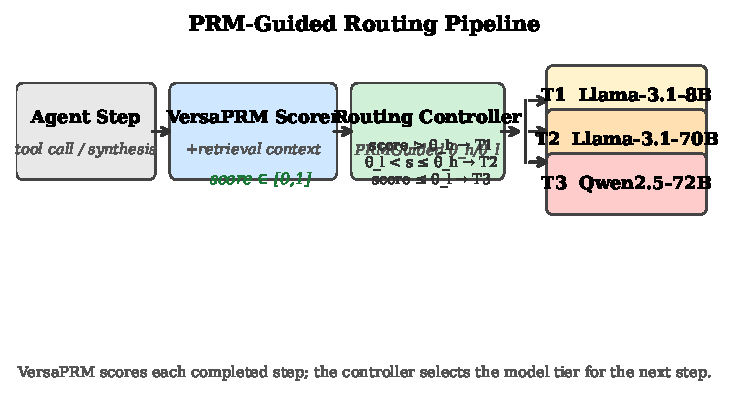
\includegraphics[width=\linewidth]{figures/fig1_system_diagram.pdf}
  \caption{PRM-Guided Routing Pipeline. VersaPRM scores each completed step;
    the controller selects the model tier for the next step.}
  \label{fig:system}
\end{figure}

% ─────────────────────────────────────────────────────────────────────────────
\section{Experiments}
% ─────────────────────────────────────────────────────────────────────────────

\paragraph{Dataset.}
AgentProcessBench~\cite{agentprocessbench2026}: 1,000 trajectories across four
datasets (hotpotqa, gaia\_dev, bfcl, tau2), 8,509 human-labeled step-quality
annotations.  We use an 800/200 train/test split (200/50 per dataset).

\paragraph{Simulation model.}
We evaluate routing via counterfactual simulation on existing trajectories~\cite{trim2026}.
Tier-$k$ outcome probabilities: $p_\text{good}(k) \in \{0.92, 0.97, 0.99\}$,
$p_\text{bad}(k) \in \{0.30, 0.65, 0.85\}$.  Task accuracy = product of
per-step success probabilities.

\subsection{Exp 1: PRM Signal Evaluation}
\label{sec:exp1}

We score all 8,509 steps with four PRMs: Qwen2.5-Math-PRM~\cite{qwenprm2025},
VersaPRM~\cite{versaprm2025}, DG-PRM~\cite{dgprm2025}, and
AgentRM~\cite{agentrm2025}.

\begin{figure}[t]
  \centering
  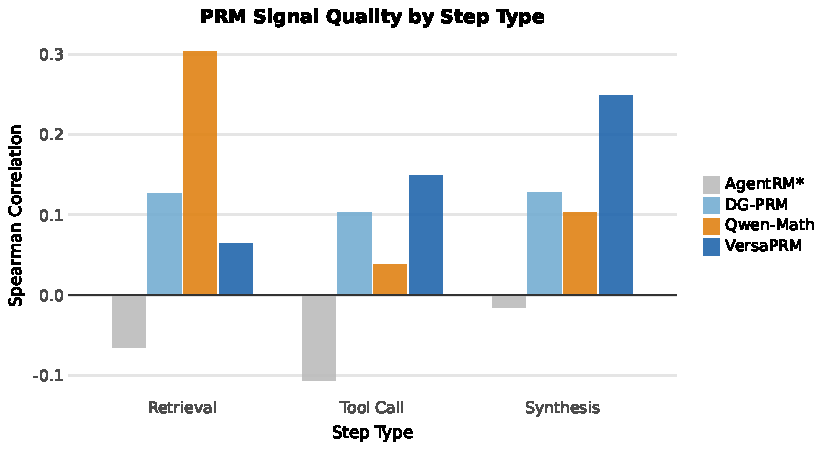
\includegraphics[width=\linewidth]{figures/fig2_prm_signal_by_step_type.pdf}
  \caption{Exp 1: Spearman correlation between PRM scores and human step labels,
    broken down by step type.  Only VersaPRM is consistently above zero.
    Qwen PRM has inverted signal on retrieval steps.  (*AgentRM weights
    released without regression head; backbone proxy used.)}
  \label{fig:signal}
\end{figure}

\cref{fig:signal} shows Spearman correlation by step type.
\textbf{VersaPRM is the only PRM with reliable step-quality signal} (global
$r_s = +0.166$, $F_1 = 0.753$, ECE $= 0.127$, step separation $= +0.064$).
Qwen2.5-Math-PRM produces inverted signal on the full dataset (step
separation $= -0.036$), confirming the math-PRM transfer gap.  AgentRM's
released weights omit the regression head; its proxy scores are near-constant.

\subsection{Exp 2: Routing Comparison}
\label{sec:exp2}

\cref{fig:pareto} shows the cost--accuracy Pareto frontier.
PRM-Guided strictly dominates TRIM at every operating point in the sweep:
$+10$ pp accuracy at matched cost (${\approx}320$k norm units), and
$21$--$26\%$ lower cost at matched accuracy levels.

BAAR over-escalates ($65\%$ of steps to Tier~3), producing higher cost than
Frontier at lower accuracy than Uniform.  DAAO degenerates to Always-Cheap
because question-length heuristics cannot discriminate agent task difficulty.

\begin{table}[t]
\small
\centering
\caption{Exp 2: Fixed-policy results (200-traj. test set).}
\label{tab:exp2}
\begin{tabular}{lrrrrr}
\toprule
Method & Acc & Cost (norm) & Esc. & AvgTier & Stab. \\
\midrule
Always-Cheap   & 0.194 & \phantom{0}70k & 0.00 & 1.00 & 1.00 \\
Uniform (T2)   & 0.388 & 316k & 0.00 & 2.00 & 1.00 \\
Frontier (T3)  & 0.617 & 633k & 1.00 & 3.00 & 1.00 \\
DAAO           & 0.194 & \phantom{0}70k & 0.00 & 1.00 & 1.00 \\
BAAR           & 0.338 & 492k & 0.65 & 2.30 & 0.81 \\
TRIM ($\theta{=}0.75$) & 0.298 & 388k & 0.47 & 2.04 & 0.56 \\
\textbf{PRM-Guided}    & \textbf{0.347} & \textbf{323k} & \textbf{0.15} & \textbf{1.94} & \textbf{0.55} \\
\bottomrule
\end{tabular}
\end{table}

\begin{figure}[t]
  \centering
  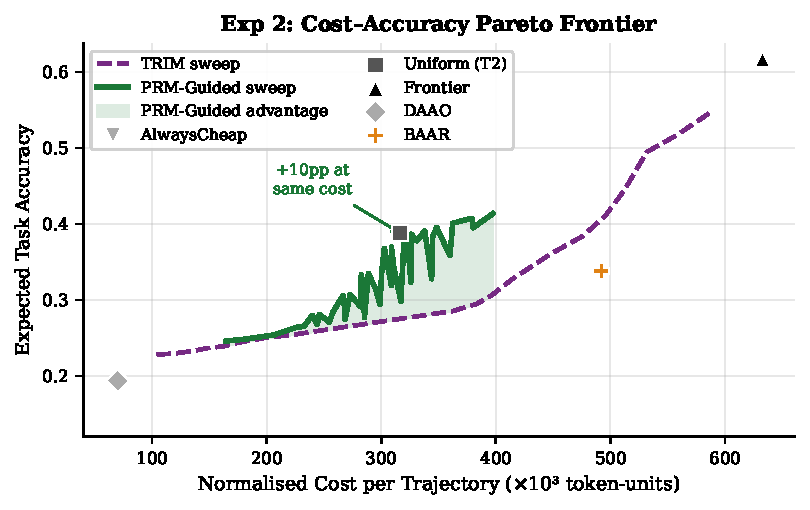
\includegraphics[width=\linewidth]{figures/fig3_pareto_frontier.pdf}
  \caption{Exp 2: Cost--accuracy Pareto frontier.  PRM-Guided (solid green)
    dominates TRIM (dashed purple) at every operating point.  Shaded region
    shows the accuracy advantage at equal cost.}
  \label{fig:pareto}
\end{figure}

\subsection{Exp 4: Domain Generalization}
\label{sec:exp4}

We train on three AgentProcessBench datasets (hotpotqa, gaia\_dev, bfcl) and
test zero-shot on tau2 (conversational banking/airline tasks).  PRM-Guided
degrades by only $-4.1$ pp ($10\%$ relative), compared to $-7.3$ pp ($16\%$)
for Uniform.  The gap between PRM-Guided and Uniform narrows from $-4.5$ pp
in-distribution to $-1.2$ pp on transfer, indicating VersaPRM's signal
generalises across agent task structures.

\subsection{Exp 10: Retrieval Context in PRM Scoring}
\label{sec:exp10}

In all prior experiments, VersaPRM scores steps using only the query and step
text---discarding retrieved passages that directly establish whether a step's
action was appropriate.  Including full retrieval context raises routing
accuracy from $0.347 \to 0.413$ ($+6.6$ pp), the largest single improvement
across all experiments.  Applying Caveman compression~\cite{jiang2023} to
retrieved passages preserves most of this gain ($0.402$, $-1.1$ pp) while
reducing retrieval context tokens by $14.8\%$.

\cref{fig:quality} summarises the routing quality analysis.

\begin{figure}[t]
  \centering
  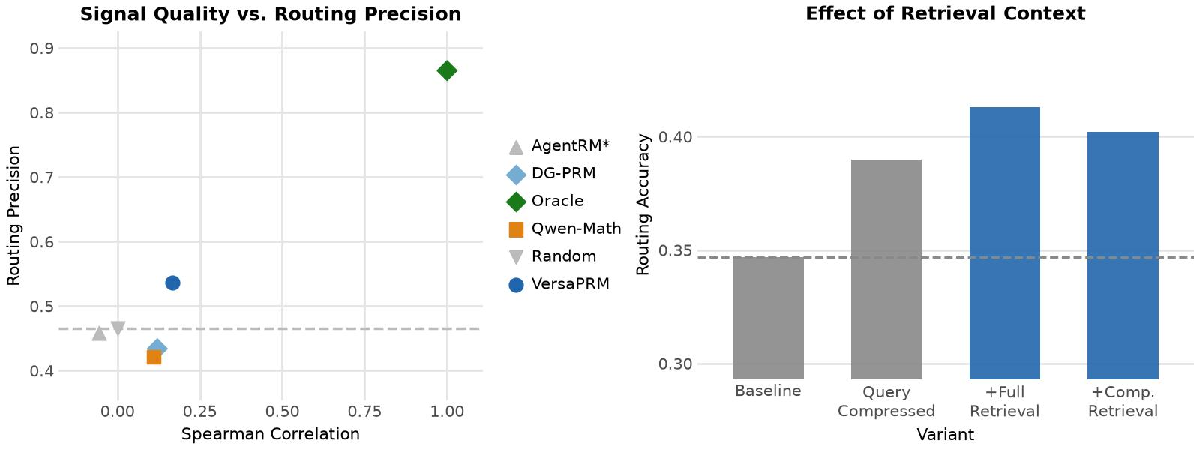
\includegraphics[width=\linewidth]{figures/fig4_routing_quality_summary.pdf}
  \caption{(a) Routing precision vs.\ Exp~1 signal quality. VersaPRM is the
    only PRM above the random baseline (dashed).
    (b) Routing accuracy under four context configurations (Exp~10).
    Including retrieval context yields $+6.6$ pp over baseline.}
  \label{fig:quality}
\end{figure}

% ─────────────────────────────────────────────────────────────────────────────
\section{Discussion and Conclusion}
% ─────────────────────────────────────────────────────────────────────────────

We have shown that multi-domain PRMs provide reliable step-quality routing
signals for heterogeneous agent pipelines, and that three-tier PRM-guided
routing strictly dominates binary TRIM routing on the cost--accuracy Pareto
frontier.  Two findings stand out beyond the main routing comparison: (1) math
PRMs do \emph{not} transfer to agent steps---Qwen2.5-Math-PRM has inverted
signal on retrieval tasks; (2) including retrieved context in PRM scoring
yields a larger routing improvement than any policy change we tested.

\textbf{Limitations.}  Results rest on a counterfactual simulation model; true
improvement depends on whether VersaPRM's correlation ($r_s = 0.166$) holds
for unseen agent policies.  AgentRM's released weights lack the regression
head; a complete comparison awaits a public release.

\textbf{Future work.}  Multi-judge disagreement routing (Exp~7) achieves
accuracy above Uniform ($+8.5$ pp at $\tau{=}0.08$), motivating a combined
signal study.  Updating the VersaPRM scorer to include retrieval context
(Exp~10a) should be the immediate next step before deploying PRM-guided
routing in production.

\begin{acks}
Research conducted under CS8903 Independent Study at Georgia Institute of
Technology, advised by Prof.\ Vijay Madisetti.
\end{acks}

\bibliographystyle{ACM-Reference-Format}
\bibliography{references}

\end{document}
